
\documentclass[12pt,a4paper]{scrartcl}

\usepackage[a4paper, left=2cm, right=1cm, bottom=1cm, top=1cm, includeheadfoot]{geometry}
\usepackage[ngerman]{babel}
\usepackage[utf8]{inputenc} % comment this if you uncomment utf8x
%\usepackage[utf8x]{inputenc} % uncomment this if there are problems with 'ä', 'ü', 'ö'
\usepackage{ucs}
\usepackage[usenames,dvipsnames]{xcolor}
\usepackage[fleqn]{amsmath}
\usepackage{amsfonts}
\usepackage{amssymb}
\usepackage{color}
\usepackage{listings}
\usepackage{hyperref}
\usepackage{amsfonts}
\usepackage{listings}
\usepackage{scrpage2}
\usepackage{graphicx}


\definecolor{mygray}{rgb}{0.9,0.9,0.9}
\lstset{language=[Visual]Basic, morekeywords={param, local}}


\lstset{
   literate={ö}{{\"o}}1
           {ä}{{\"a}}1
           {ü}{{\"u}}1
           {ß}{{\ss}}1
           {é}{{\'e}}1,
   inputencoding=ansinew,
   extendedchars=true,
   basicstyle=\scriptsize\ttfamily,
   numberstyle=\scriptsize,
   breaklines=true,
   tabsize=2,
   numbersep=5pt
}
\lstdefinestyle{customcpp}{
   language=C++,
   backgroundcolor=\color{mygray},
   numbers=left,
   keywordstyle=\color{blue}\bfseries,
   stringstyle=\color{BrickRed}\ttfamily,
   commentstyle=\color{OliveGreen}\ttfamily,
   showspaces=false,
   showstringspaces=false,
   showtabs=false
}
\lstdefinestyle{customoutput}{
   backgroundcolor=\color{mygray},
   numbers=none,
   showspaces=false,
   showtabs=false
}

\newcommand{\sourceCode}[1]{\lstinputlisting[style=customcpp]{#1}} %beinhaltet alle benötigten Packages etc.
\begin{document}
\graphicspath{{./}}

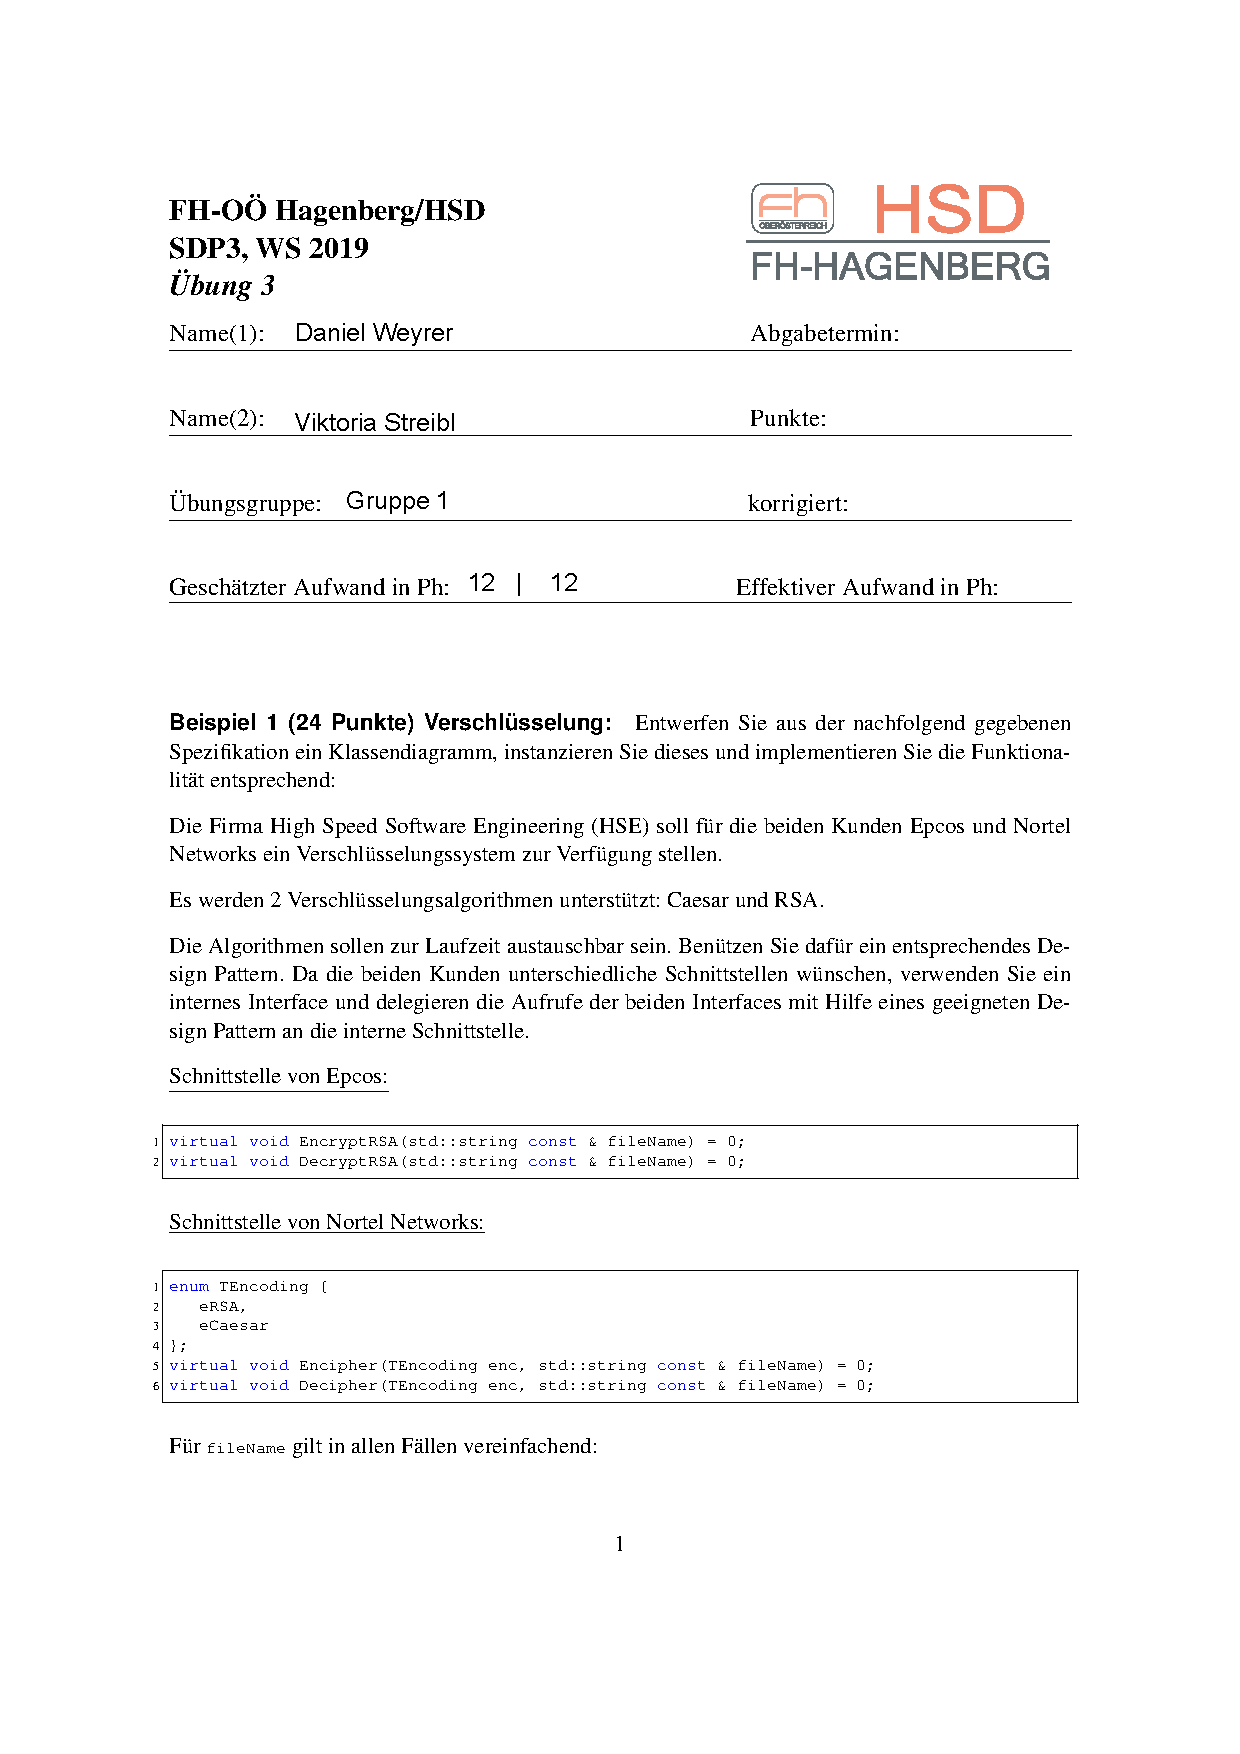
\includepdf[pages=-]{Angabe.pdf}

\title{SDP - Exercise 02} % Übungsname und Nummer angeben
\subtitle{winter semester 2019/20} % Semester angeben oder auskommentieren, falls nicht erwünscht
\author{
Viktoria Streibl - S1810306013\\
  Daniel Weyrer - S1820306044
} % Autorenname
\date{\today} % Das heutige Datum automatisch einfügen

\maketitle % Titelseite erstellen

\newpage
\tableofcontents % Inhaltsverzeichnis erstellen
\newpage

\ihead{Viktoria Streibl}
\ohead{Daniel Weyrer}
\chead{SDP3-UE Uebung 02}

\section{Organizational}
\subsection{Team}
\begin{itemize}
	\item Viktoria 	Streibl 		- 	S1810306013
	\item Daniel 	Weyrer		-	S1820306044
\end{itemize}

\subsection{Roles and responsibilities}

\subsubsection{Jointly}
\begin{itemize}
	\item planning
	\item Documentation
	\item Systemdocumentation
	\item Class Diagram
\end{itemize}

\subsubsection{Viktoria Streibl}
\begin{itemize}
	\item Main Class Company
	\item Interface ICompany
	\item Testdriver Client
	\item Main Testdriver
	
\end{itemize}

\subsubsection{Daniel Weyrer}
\begin{itemize}
	\item Base Class for Employee
	\item Derived Classes
		\subitem Class Commission Worker
		\subitem Class Hourly Worker
		\subitem Class Pieces Worker
		\subitem Class Boss
\end{itemize}

\subsection{Effort}

\subsubsection {Viktoria Streibl}
\begin{itemize}
	\item estimated: 10ph 
	\item actually: 11 ph
\end{itemize}

\subsubsection {Daniel Weyrer}
\begin{itemize}
	\item estimated: 10 ph 
	\item actually: 11 ph
\end{itemize}

\section{Requirenment Definition(System Specification)}
It was a company desired the various types of employees includes, such as commission worker, hourly worker, pieces worker and boss. Each employee type should also include and output some key data such as name, SSN, date of joining, salary and birthday. In addition, each company has to ouput the name and location.
Any number of employees can be added and deleted in the programm, but the client is not allowed to do so. It is possible to search for employees by nickname as well as by the type. The Client can also get all produces and all sold pieces.

\section{System Design}
\subsection{Classdiagram}
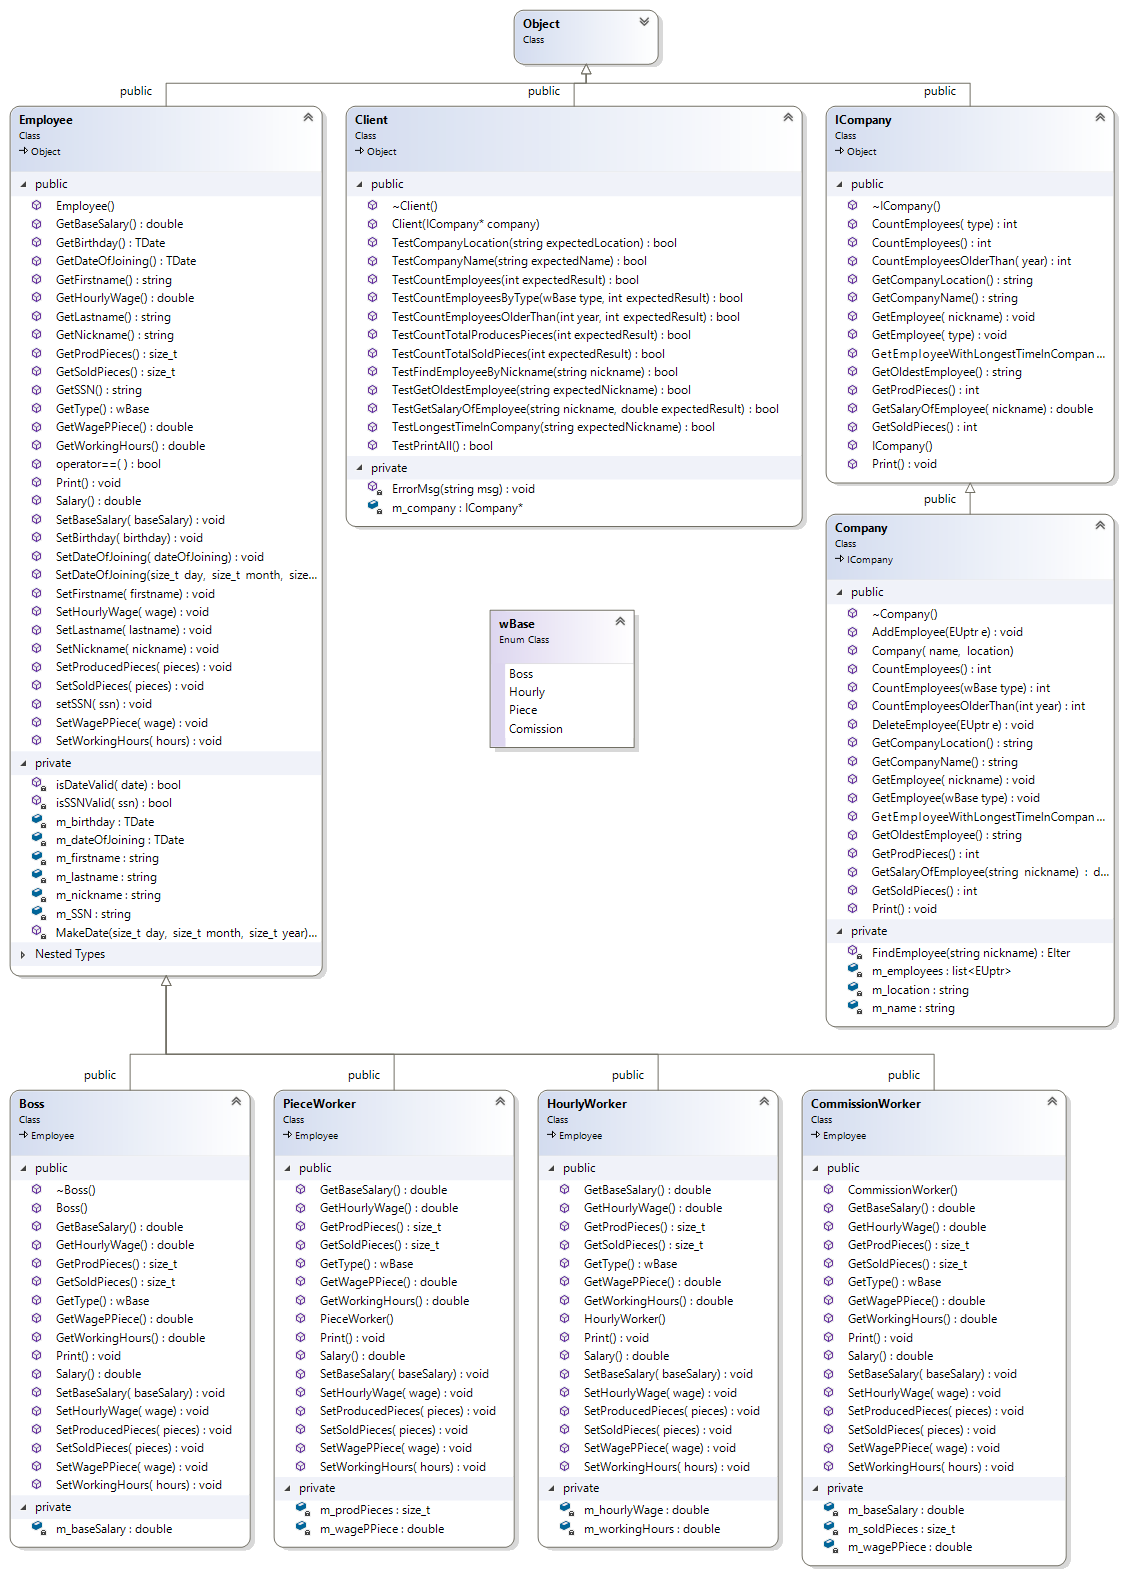
\includegraphics[scale=0.6]{ClassDiagram}

\subsection{Design Decisions}
\subsubsection{cTor`s Derived Classes (Base: Employee)}
The cTor`s of the derived classes set every wage and number to 0, to identify uninitialized variables (as the Salary is 0 when one of the two parameters are 0!).
\subsubsection{isDateValid}
The Date get`s it`s validation in two steps:
\begin{itemize}
	\item correct date-syntax
	\item is the entered date in a valid range
\end{itemize}
The first step is achieved by checking with number of days in each month while taking care of the leapyears!

The second step is done by comparing the current date with the entered date (which has to be in the past!).
\subsubsection{Search Employee}
Employee is searched by nickname because it has to be unique. To be sure that the nickname is unique we check it while adding new employee.

\section{Component Design}
\subsection{Class Client}
The Client simulate a person which use the interface.
The following functions tests the functionality:
\begin{itemize}
	\item Tests the company name
	\item Tests the company location
	\item Tests if it is possible to find a employee by nickname
	\item Tests if the employee which is search by his nickname is correct
	\item Counts all employees and check if it is correct
	\item Counts all employees of one type and check it
	\item Counts all produced pieces and check them
	\item Counts all sold pieces and check them
	\item Count how many employees are older than a specific year and check it
	\item Tests if the salary of an employee is correct
	\item Tests if the oldest employee is correct
	\item Check for the employee with is the oldest member
	\item Print all data of company and employees
\end{itemize}

All these methods are only for testing the functionality of Company. Furthermore, the Client gets the company with the constructor as ICompany.

\subsection{Class ICompany}
Is an interface which is used by the Client.
It contains the following functions:
\begin{itemize}
	\item Get the company name
	\item Get the company location
	\item Get an employee by nickname
	\item Get all employees of the same type
	\item Get all sold pieces
	\item Get all produced pieces
	\item Get salary of an employee
	\item Get oldest employee
	\item Get employee with the longest time in the company
	\item Count all employees in the company
	\item Count all employees with the same type
	\item Count all employees which are older than a specific year
	\item Output all employees in the company and some general data
\end{itemize}

The ICompany is the interface between an client and the company. The Client is not allowed to manipulate the employees.
It defines the methods with can be used by the client.

"GetCompanyName", returns the name of the company.
"GetCompanyLocation", returns the location of the company.
"GetEmployee", can be used with the nickname or the type and returns the employees.
"GetSoldPieces", counts all pieces which are sold by the company.
"GetProdPieces", counts all pieces which are produces by the employees.
"GetSalaryOfEmployee", returns the salaray of an employee.
"GetOldestEmployee", returns the oldest employee.
"GetEmployeeWithLongestTimeInCompany", returns the nickname of the employee with the oldes join in date
"CountEmployees", returns the number of employees in the company, can be specifified with type.
"CountEmployeesOlderThan", counts how many amployees are older than a specific year.
"Print", outputs the name and location of the company, as well as all employees.
\newpage

\subsection{Class Company}
Manages all employees in the company. It implements the interface ICompany.
It contains the following functions:
\begin{itemize}
	\item Add a new Employee
	\item Remove a Employee
	\item All functions from ICompany
	\item findEmployee
\end{itemize}

The Company class manages all Employees. It uses unique pointers stored in a vector, to avoid shallow-copies.
With the method "AddEmploye" a new employee can be created. Should a employee already exist with the same nickname. So this employee is not stored and an error message output.
"DeleteEmployee" deletes a employee. If none is stored with the nickname an exception get`s thrown and caught in the same method.
The private function "FindEmployee", loop through the list and checks if there is any employee with the specific nickname.

\subsection{Class Employee}
Is the base class of all employee types.
It contains the following functions:
\begin{itemize}
	\item Contains the Get and Set pure virtual functions for the derived classes
	\item Overloaded Output-Operator for date-struct
\end{itemize}

\subsection{Class CommissionWorker}
This class represents a commission worker.
\begin{itemize}
	\item The ComissionWorker gets a base Salary and a commssion for every sold piece
\end{itemize}

\subsection{Class HourlyWorker}
This class represents a hourly worker.
\begin{itemize}
	\item contains workinghours and the hourly wage the worker gets for each hour.
\end{itemize}

\subsection{Class PiecesWorker}
This class represents a pieces worker.
\begin{itemize}
	\item saves number of produced pieces and the wage the worker gets for every piece he produces
	
\end{itemize}

\subsection{Class Boss}
This class represents a boss.
\begin{itemize}
	\item BaseSalary, as it`s independent from the Boss' actions!
\end{itemize}

\subsection{TestDriver}
The Testdriver test alle functions of the Client. It adds commisson worker, hourly worker, pieces worker and a boss.
The functions "TestLinzAG", "TestSequality" and "TestTractive" call the testing functions of client and check if everything worked.
The test-functions in Client returns a bool. If the bool returns false something didn't pass and this Testcase cannot get valid again.
It ouputs a error message if there was no successful run.

\newpage
\section{Test Protocol}
It has been tested in the file "TestDriver", the following points have been tested:
\begin{itemize}
	\item get name of the company
	\item get location of the company
	\item count all employees in the company
	\item find an employee by his nickname
	\item searching for the oldest employee
	\item count all employees older than 1990.
	\item get the employee with the oldest joining date.
	\item count all employees by the same type
	\item count all sold pieces this month
	\item test the salary of a employee
\end{itemize}

\subsection{Console Output}
\sourceCode{./CalcSalary/output.txt}
\newpage

\section{Source Code}


\subsection{Class Client}
\subsubsection{Client.h}
\sourceCode{./CalcSalary/CalcSalary/Client.h}
\newpage
\subsubsection{Client.cpp}
\sourceCode{./CalcSalary/CalcSalary/Client.cpp}
\newpage
\subsection{Interface ICompany}
\subsubsection{ICompany.h}
\sourceCode{./CalcSalary/CalcSalary/ICompany.h}
\newpage
\subsection{Class Company}
\subsubsection{Company.h}
\sourceCode{./CalcSalary/CalcSalary/Company.h}
\subsubsection{Company.cpp}
\sourceCode{./CalcSalary/CalcSalary/Company.cpp}
\newpage
\subsection{Class Employee}
\subsubsection{Employee.h}
\sourceCode{./CalcSalary/CalcSalary/Employee.h}
\newpage
\subsubsection{Employee.cpp}
\sourceCode{./CalcSalary/CalcSalary/Employee.cpp}

\newpage
\subsection{Class CommissionWorker}
\subsubsection{CommissionWorker.h}
\sourceCode{./CalcSalary/CalcSalary/CommissionWorker.h}
\newpage
\subsubsection{CommissionWorker.cpp}
\sourceCode{./CalcSalary/CalcSalary/CommissionWorker.cpp}

\subsection{Class HourlyWorker}
\subsubsection{HourlyWorker.h}
\sourceCode{./CalcSalary/CalcSalary/HourlyWorker.h}
\newpage
\subsubsection{HourlyWorker.cpp}
\sourceCode{./CalcSalary/CalcSalary/HourlyWorker.cpp}

\subsection{Class PieceWorker}
\subsubsection{PieceWorker.h}
\sourceCode{./CalcSalary/CalcSalary/PieceWorker.h}
\newpage
\subsubsection{PieceWorker.cpp}
\sourceCode{./CalcSalary/CalcSalary/PieceWorker.cpp}

\subsection{Class Boss}
\subsubsection{Boss.h}
\sourceCode{./CalcSalary/CalcSalary/Boss.h}
\newpage
\subsubsection{Boss.cpp}
\sourceCode{./CalcSalary/CalcSalary/Boss.cpp}

\subsubsection{TestDriver.cpp}
\sourceCode{./CalcSalary/CalcSalary/TestDriver.cpp}

% Um Quellcode einzufügen einfach diesen Befehl verwenden:
%\sourceCode{Relativer/Pfad/zum/SourceCode.Endung}

\end{document}